\documentclass[../main.tex]{subfiles}
\begin{document}
    Hauptpunkte der Besprechung:
    \begin{itemize}
        \item Es gibt (Kern-)spins, welche sich durch Summierung der Protonenspins ergeben. Prominentes Beispiel ist Wasserstoff.
        \item Wir wollen den Effekt der Auslenkung des Spinvektors gegenüber eines Magnetfeldes (kontaktlos) untersuchen. 
        \item Der Spinvektor präzidiert mit der \emph{Lamorfrequenz} $\omega_L$. Diese ist (u.a.) abhängig von der Magnetfeldstärke. Wenn in einem Material alle solchen in Phase präzidieren, dann addiert sich das so erzeugte Magnetfeld konstruktiv. 
        \item Das Magnetfeld soll möglichst homogen sein, wir benutzen das Erdmagnetfeld.
        \item Man bezeichnet den Prozess mit MRI. Bei dem Aufbau handelt es sich um drei Spulen. Es gibt eine Messspule, eine Gradientenspule und eine Polarisationsspule.
        \item Wir untersuchen verschiedene Proben und wollen (u.a.) die Elemente identifizieren. 
    \end{itemize}
    \begin{figure}[H]
        \centering
        \begin{subfigure}[b]{0.32\textwidth}
            \centering
            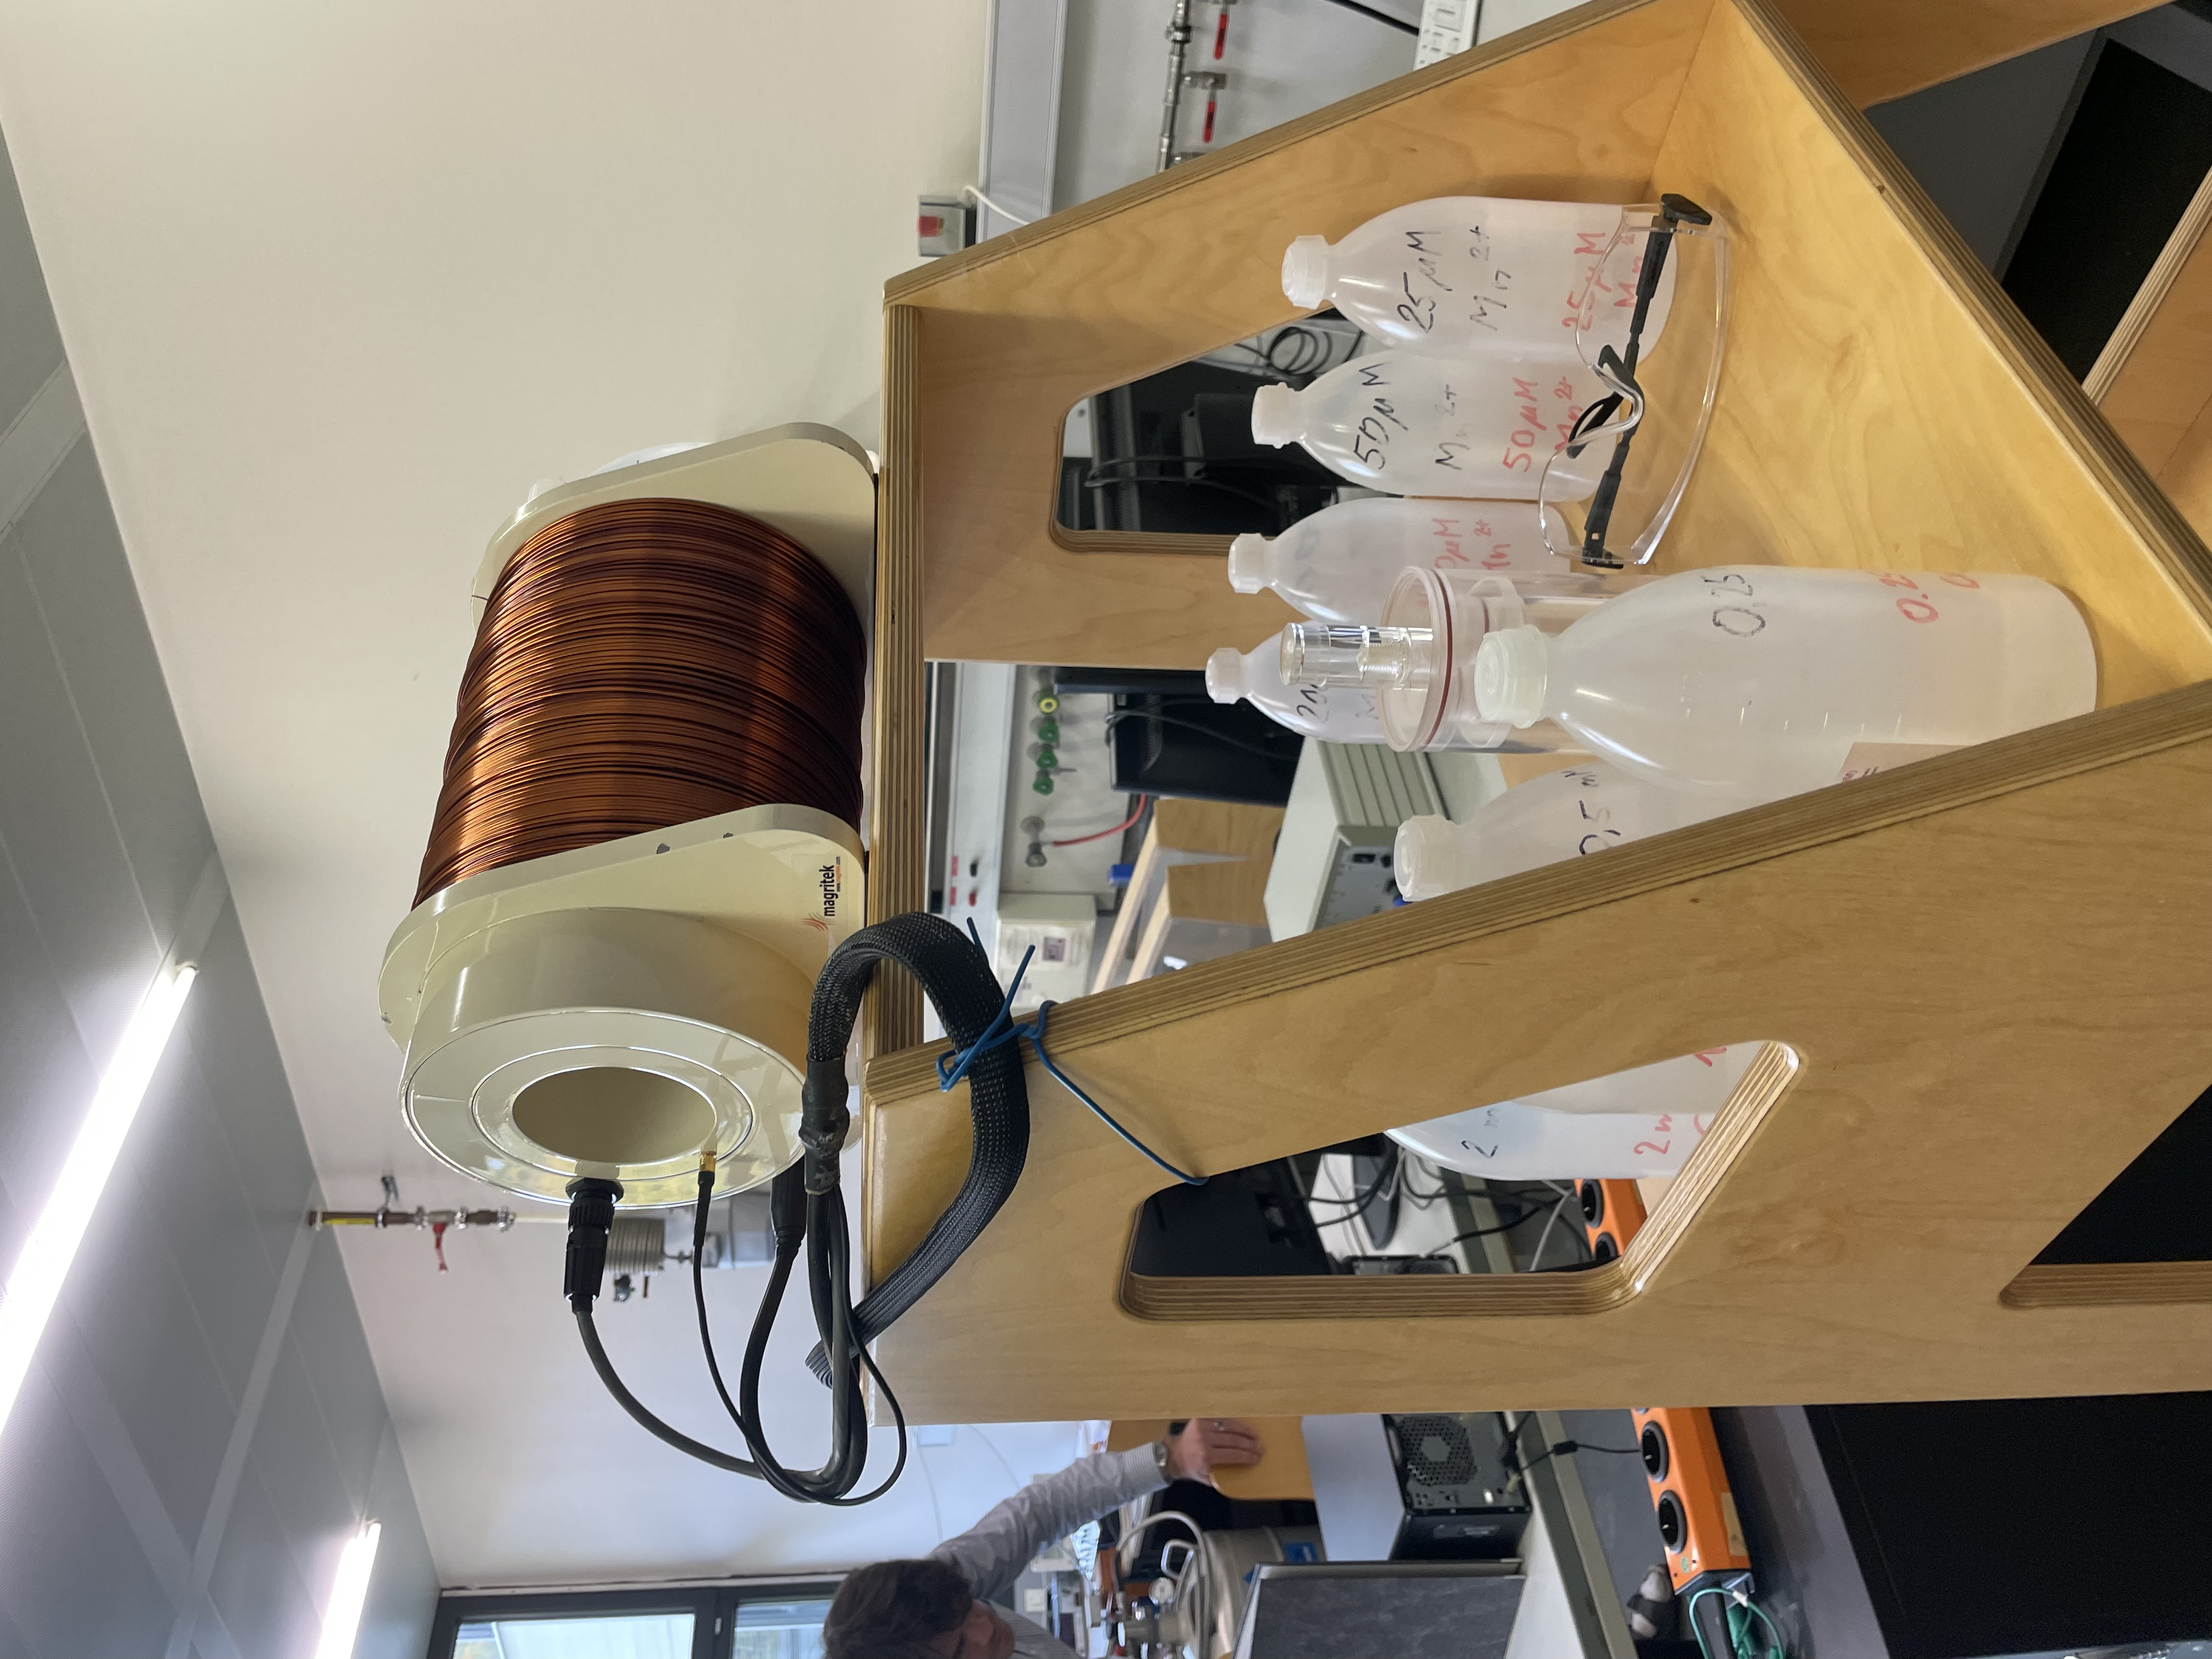
\includegraphics[width=5cm,angle=270]{Bilddateien/1B3CD638-A034-4302-B2E8-81D900DB3547.jpeg}
            \caption{Versuchsaufbau}
            \label{fig:Versuchsaufbau}
        \end{subfigure}
        \
        \begin{subfigure}[b]{0.32\textwidth}
            \centering
            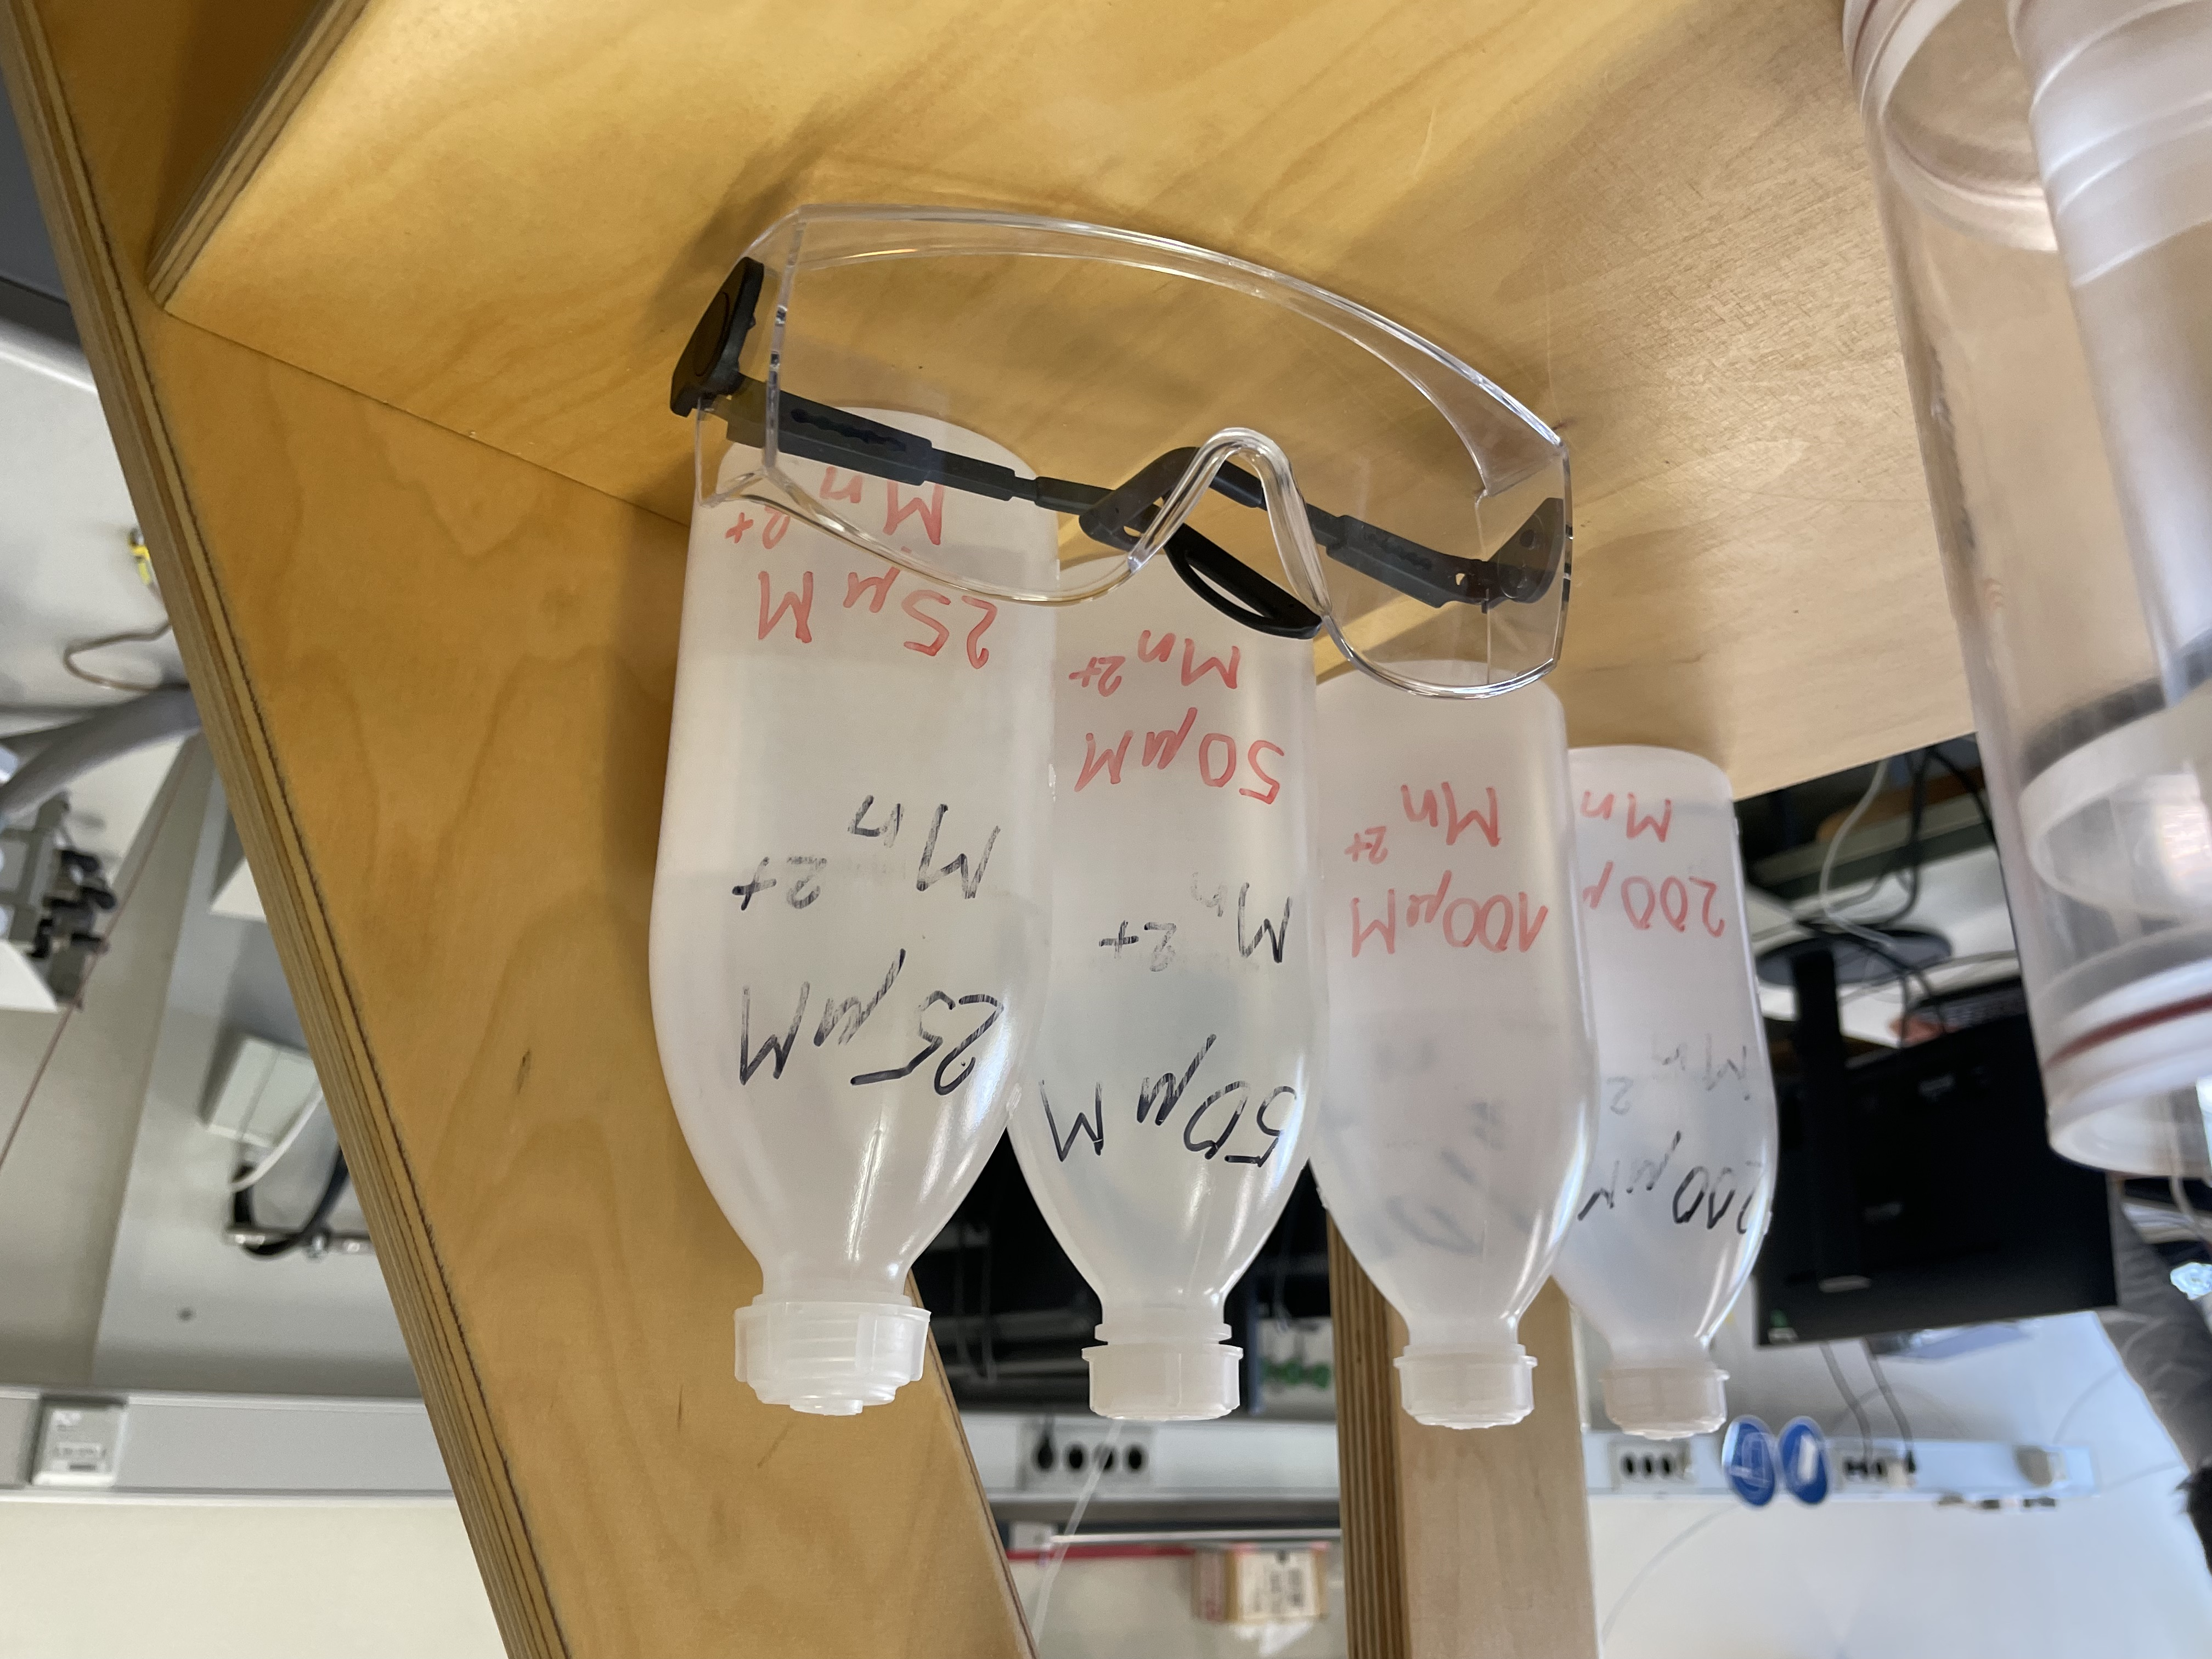
\includegraphics[width=4cm,angle=180]{Bilddateien/2D6634FA-11FA-4A5E-9C13-93C4F30340D7.jpeg}
            \caption{Proben}
            \label{fig:Proben}
        \end{subfigure}
        \
        \begin{subfigure}[b]{0.32\textwidth}
            \centering
            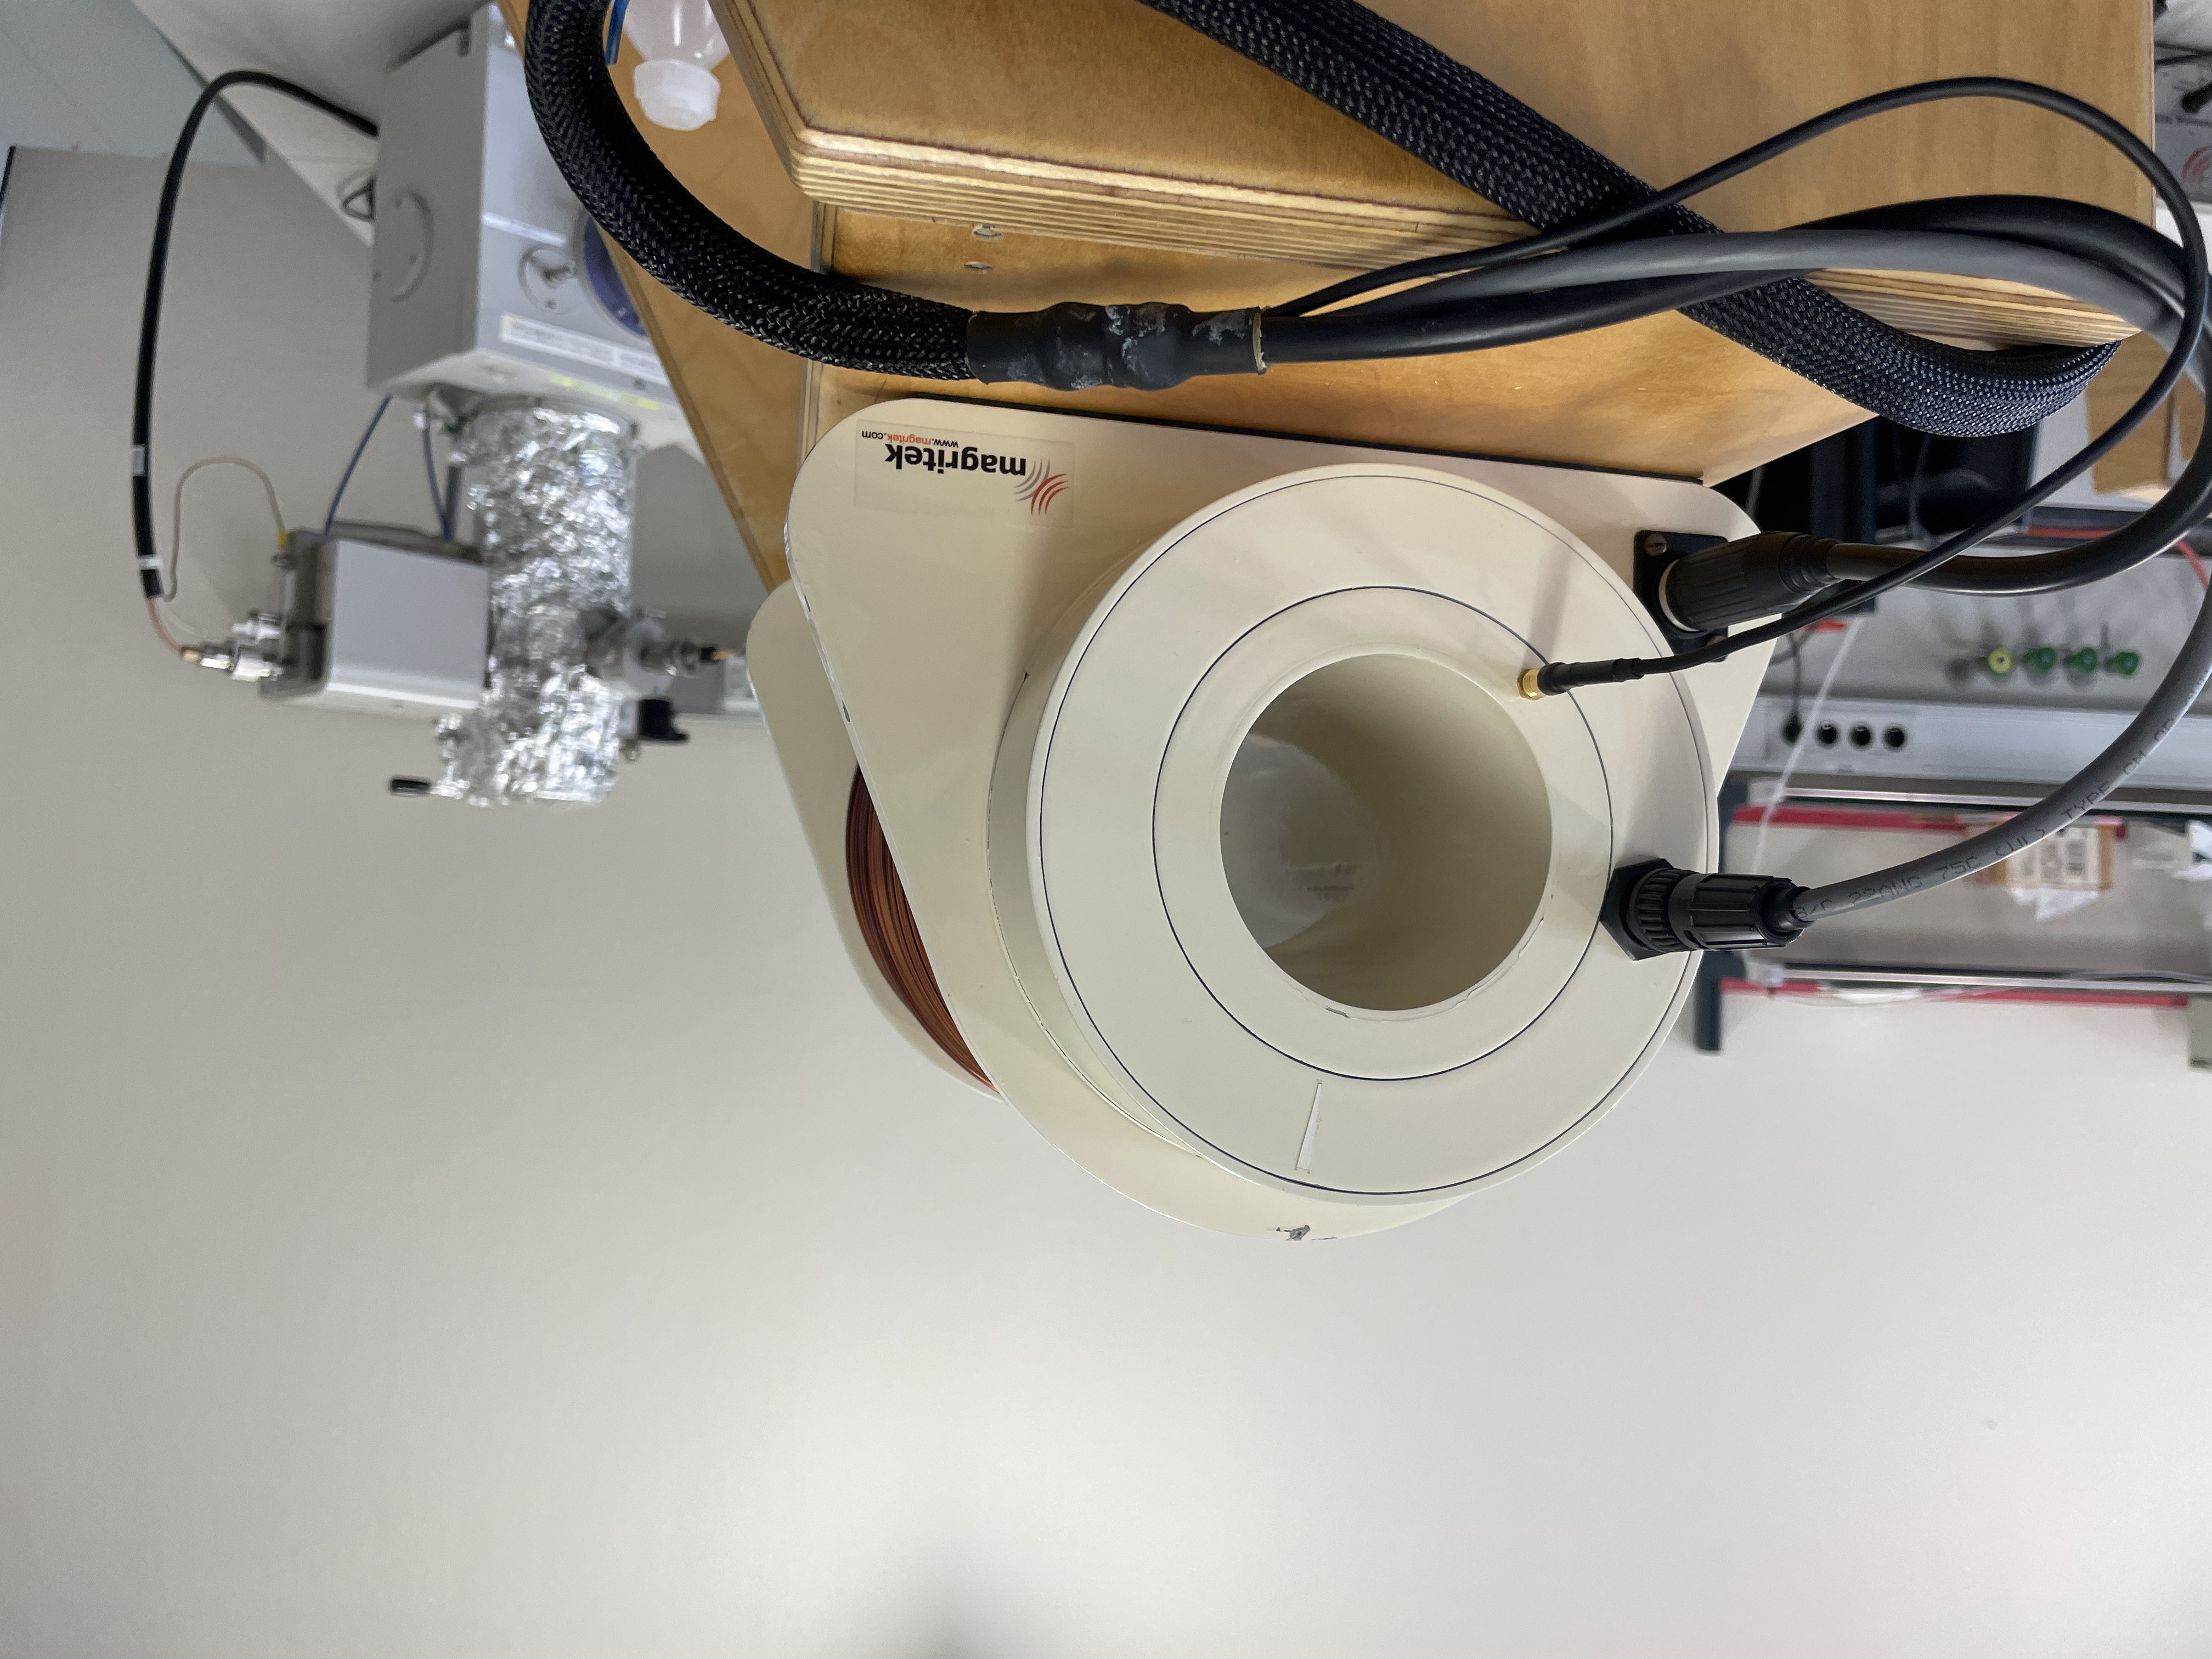
\includegraphics[width=4cm,angle=180]{Bilddateien/4D7C3F5A-8634-4ED8-802E-E878DEABC504.jpeg}
            \caption{Spulen außen}
            \label{fig:SpulenAussen}
        \end{subfigure}
    \end{figure}
\end{document}